\section{Modelling of Handover Manipulations}

- present a short version of the deceleration phase (previous paper)
- explain why you decide to resort to this new approach

\begin{figure}[t]
\tikzset{every picture/.style={line width=0.75pt}} %set default line width to 0.75pt        

\begin{tikzpicture}[x=0.75pt,y=0.75pt,yscale=-1,xscale=1]
%uncomment if require: \path (0,394); %set diagram left start at 0, and has height of 394

%Shape: Rectangle [id:dp8171705286563367] 
\draw   (0.5,192.38) -- (48.57,192.38) -- (48.57,219.61) -- (0.5,219.61) -- cycle ;
%Shape: Rectangle [id:dp16137444864977923] 
\draw   (95.51,2.5) -- (224.25,2.5) -- (224.25,20.16) -- (95.51,20.16) -- cycle ;
%Shape: Rectangle [id:dp6063905810492368] 
\draw  [dash pattern={on 4.5pt off 4.5pt}] (62.63,39.3) -- (250.83,39.3) -- (250.83,161) -- (62.63,161) -- cycle ;
%Image [id:dp43598404181394723] 
\draw (156.73,100.15) node  {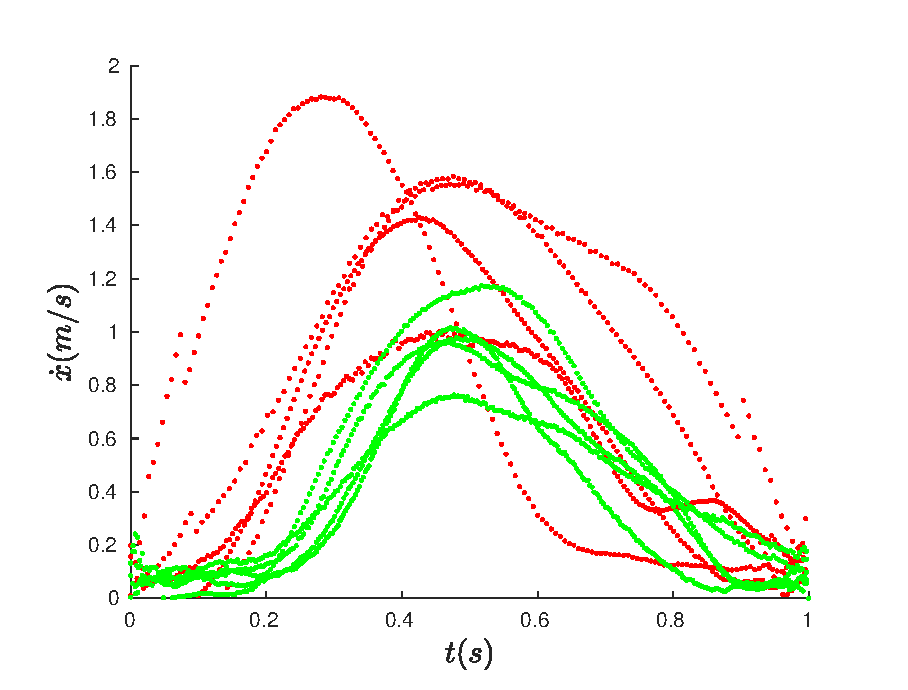
\includegraphics[width=141.15pt,height=91.28pt]{Images/vel_distance_plot.eps}};
%Shape: Rectangle [id:dp7136803259697821] 
\draw  [color={rgb, 255:red, 255; green, 255; blue, 255 }  ,draw opacity=0 ][fill={rgb, 255:red, 245; green, 166; blue, 35 }  ,fill opacity=0.55 ] (156.73,39.3) -- (250.83,39.3) -- (250.83,161) -- (156.73,161) -- cycle ;
%Shape: Rectangle [id:dp4989299581398505] 
\draw  [color={rgb, 255:red, 255; green, 255; blue, 255 }  ,draw opacity=0 ][fill={rgb, 255:red, 75; green, 87; blue, 211 }  ,fill opacity=0.39 ] (62.63,39.3) -- (156.73,39.3) -- (156.73,161) -- (62.63,161) -- cycle ;
%Straight Lines [id:da2860186468382656] 
\draw    (156.82,21.39) -- (156.85,34.49) -- (156.86,35.07) ;
\draw [shift={(156.87,37.07)}, rotate = 269.53] [color={rgb, 255:red, 0; green, 0; blue, 0 }  ][line width=0.75]    (7.65,-3.43) .. controls (4.86,-1.61) and (2.31,-0.47) .. (0,0) .. controls (2.31,0.47) and (4.86,1.61) .. (7.65,3.43)   ;
%Rounded Rect [id:dp6443750059991944] 
\draw   (85.68,191.92) .. controls (85.68,186.88) and (89.77,182.8) .. (94.81,182.8) -- (219.21,182.8) .. controls (224.25,182.8) and (228.34,186.88) .. (228.34,191.92) -- (228.34,219.3) .. controls (228.34,224.34) and (224.25,228.43) .. (219.21,228.43) -- (94.81,228.43) .. controls (89.77,228.43) and (85.68,224.34) .. (85.68,219.3) -- cycle ;
%Rounded Rect [id:dp0531242957100273] 
\draw   (93.69,194.2) .. controls (93.69,190.14) and (96.99,186.84) .. (101.05,186.84) -- (145.23,186.84) .. controls (149.29,186.84) and (152.59,190.14) .. (152.59,194.2) -- (152.59,216.28) .. controls (152.59,220.35) and (149.29,223.64) .. (145.23,223.64) -- (101.05,223.64) .. controls (96.99,223.64) and (93.69,220.35) .. (93.69,216.28) -- cycle ;
%Rounded Rect [id:dp10795879107477857] 
\draw   (163.25,195.31) .. controls (163.25,191.45) and (166.38,188.32) .. (170.24,188.32) -- (215.15,188.32) .. controls (219.01,188.32) and (222.15,191.45) .. (222.15,195.31) -- (222.15,216.28) .. controls (222.15,220.14) and (219.01,223.27) .. (215.15,223.27) -- (170.24,223.27) .. controls (166.38,223.27) and (163.25,220.14) .. (163.25,216.28) -- cycle ;
%Straight Lines [id:da9553234338793252] 
\draw    (52.94,206.85) -- (80.94,206.73) ;
\draw [shift={(80.94,206.73)}, rotate = 180] [color={rgb, 255:red, 0; green, 0; blue, 0 }  ][line width=0.75]    (8.74,-3.92) .. controls (5.56,-1.84) and (2.65,-0.53) .. (0,0) .. controls (2.65,0.53) and (5.56,1.84) .. (8.74,3.92)   ;
%Straight Lines [id:da8975459341516769] 
\draw    (231.22,207.35) -- (248.04,207.6) ;
\draw [shift={(250.04,207.63)}, rotate = 180.85] [color={rgb, 255:red, 0; green, 0; blue, 0 }  ][line width=0.75]    (8.74,-3.92) .. controls (5.56,-1.84) and (2.65,-0.53) .. (0,0) .. controls (2.65,0.53) and (5.56,1.84) .. (8.74,3.92)   ;
%Rounded Rect [id:dp6783697061768484] 
\draw   (254.14,195.79) .. controls (254.14,192.08) and (257.15,189.07) .. (260.86,189.07) -- (301.14,189.07) .. controls (304.85,189.07) and (307.86,192.08) .. (307.86,195.79) -- (307.86,215.95) .. controls (307.86,219.67) and (304.85,222.68) .. (301.14,222.68) -- (260.86,222.68) .. controls (257.15,222.68) and (254.14,219.67) .. (254.14,215.95) -- cycle ;
%Straight Lines [id:da7778502429910122] 
\draw    (309.58,206.76) -- (320.37,206.83) ;
\draw [shift={(322.37,206.84)}, rotate = 180.37] [color={rgb, 255:red, 0; green, 0; blue, 0 }  ][line width=0.75]    (8.74,-3.92) .. controls (5.56,-1.84) and (2.65,-0.53) .. (0,0) .. controls (2.65,0.53) and (5.56,1.84) .. (8.74,3.92)   ;
%Straight Lines [id:da060082135680290416] 
\draw    (155.97,163.81) -- (156,176.9) ;
\draw [shift={(156,178.9)}, rotate = 269.87] [color={rgb, 255:red, 0; green, 0; blue, 0 }  ][line width=0.75]    (8.74,-2.63) .. controls (5.56,-1.12) and (2.65,-0.24) .. (0,0) .. controls (2.65,0.24) and (5.56,1.12) .. (8.74,2.63)   ;
%Straight Lines [id:da8234214050961214] 
\draw    (66.94,206.79) -- (67.37,242.34) ;
%Straight Lines [id:da5201978982400552] 
\draw    (283.93,242.41) -- (283.75,227.01) ;
\draw [shift={(283.72,225.01)}, rotate = 449.31] [color={rgb, 255:red, 0; green, 0; blue, 0 }  ][line width=0.75]    (8.74,-3.92) .. controls (5.56,-1.84) and (2.65,-0.53) .. (0,0) .. controls (2.65,0.53) and (5.56,1.84) .. (8.74,3.92)   ;
%Straight Lines [id:da7606688623528574] 
\draw    (67.37,242.34) -- (283.93,242.41) ;

% Text Node
\draw (239.25,42.92) node [anchor=north west][inner sep=0.75pt]  [font=\scriptsize] [align=left] {1};
% Text Node
\draw (66.3,41.74) node [anchor=north west][inner sep=0.75pt]  [font=\scriptsize,rotate=-359.78] [align=left] {2};
% Text Node
\draw (98.28,192.99) node [anchor=north west][inner sep=0.75pt]  [font=\scriptsize] [align=left] {\begin{minipage}[lt]{34.85pt}\setlength\topsep{0pt}
\begin{center}
Careful \\Behaviour
\end{center}

\end{minipage}};
% Text Node
\draw (165.25,194.44) node [anchor=north west][inner sep=0.75pt]  [font=\scriptsize] [align=left] {\begin{minipage}[lt]{38.82pt}\setlength\topsep{0pt}
Not Careful
\begin{center}
Behaviour
\end{center}

\end{minipage}};
% Text Node
\draw (263.36,193.57) node [anchor=north west][inner sep=0.75pt]  [font=\scriptsize] [align=left] {\begin{minipage}[lt]{26.52pt}\setlength\topsep{0pt}
\begin{center}
Belief \\System
\end{center}

\end{minipage}};
% Text Node
\draw (234.93,190.43) node [anchor=north west][inner sep=0.75pt]  [font=\small]  {$Y$};
% Text Node
\draw (152.65,229.17) node [anchor=north west][inner sep=0.75pt]  [font=\small]  {$\dot{x}$};
% Text Node
\draw (85.38,168.08) node [anchor=north west][inner sep=0.75pt]  [font=\footnotesize] [align=left] {Model};
% Text Node
\draw (254.08,175.6) node [anchor=north west][inner sep=0.75pt]  [font=\footnotesize] [align=left] {Classifier};
% Text Node
\draw (95.32,21.79) node [anchor=north west][inner sep=0.75pt]  [font=\footnotesize] [align=left] {Dataset};
% Text Node
\draw (95.51,5.5) node [anchor=north west][inner sep=0.75pt]  [font=\footnotesize,rotate=-359.96,xslant=0] [align=left] {Human Demonstrations};
% Text Node
\draw (4.9,199.72) node [anchor=north west][inner sep=0.75pt]  [font=\footnotesize] [align=left] {Human};
\
\end{tikzpicture}
  \caption{The birds}
  \label{fig:diagram}
\end{figure}


This here Figure \ref{fig:diagram}
Let $x \in D \subset \mathbb{R}^{+}$ denote the distance of the human wrist towards the handover meeting point. 

\subsection{Deceleration Phase}

Consider a behavior encoded as a state-dependent dynamical system (DS)
%
\begin{equation}
\dot{x} = \pmb{\textnormal{f}}(x)
\label{eq:1}
\end{equation}
where $\pmb{\textnormal{f}}:\mathbb{R}^{+} \to \mathbb{R}^{+}$ is a continuous and continuously differentiable function, with a single equilibrium point ${\dot{x}_d}^* = \pmb{\textnormal{f}}(x^*)$. $x^{*}$ is set at the origin and it is globally asymptotic stable such that $\dot{x}^* = \textnormal{f}(x^{*}) = 0$ which is guaranteed under a Lyapunov function $V(x):\mathbb{R}^{+} \rightarrow \mathbb{R}^{+}$.

Our approach defines each ``carefulness'' condition, \textit{careful} and \textit{not careful}, as two distinct DS. Each DS is encoded using Gaussian Mixture Models (GMM) which defines a joint distribution function $\mathcal{P}({{x}^{t}}_n, {\dot{x}^{t}}_n | \Theta) = \sum_{k=1}^{K} \pi^{k} \mathcal{N}({{x}^{t}}_n, {\dot{x}^{t}}_n, \mu^{k}, \Sigma^{k})$ over the data as mixture of $K$ Gaussian distributions \cite{khansari2011learning}, where $\pi^{k}$, $\mu^{k}$, and $\Sigma^{k}$ are, respectively, the prior component, mean, and covariance matrix of the $k$th Gaussian. $x_n^t$ is $n$th trajectory of $x$ at time $t$, and $\dot{x}_n^t$ is its derivative. Fig. \ref{fig:motion} illustrates the position ($x$) and velocity ($\dot{x}$) relations for \textit{careful} and \textit{not careful} motions. To compute the DS from Eq. (\ref{eq:1}) the posterior mean of $\mathcal{P}({\dot{x}^{t}}_n|{{x}^{t}}_n)$ is estimated which approximates it to:
%
\begin{equation}
\hat{\dot{x}} = \sum_{n=1}^{K} h^{k}(x) (\Sigma^{k}_{\dot{x}x}(\Sigma^{k}_{xx})^{-1} (x - \mu^{k}_{x}) + \mu^{k}_{\dot{x}})
\label{eq:2}
\end{equation}
where $h^{k}(x) = \frac{\pi^{k} \mathcal{N}({{x}^{t}}, {\dot{x}^{t}}, \mu^{k}, \Sigma^{k})}{\sum_{i=1}^{K} \pi^{k} \mathcal{N}({{x}^{t}}_n, {\dot{x}^{t}}_n, \mu^{i}, \Sigma^{i})}$, $h^{k}(x) > $ 0, and $\sum_{n=1}^{K} h^{k}(x)$ = 1. The GMMs are computed using the stable estimator of dynamical systems (SEDS) approach \cite{khansari2011learning}. 

- mention limitations of this approach. The model is focused on the latter stage of the manipulation hence the recognition happens later. The models did not provide useful results for regions outside of the learned models. When testing the generated velocities for both models were very similar not allowing the classifier to distinguish between the two. 

\subsection{Acceleration Phase}

- present the new approach of the acceleration phase

- show the results of the table of deceleration vs acceleration

\subsection{Classification}

\subsection{Comparing the two approaches}

\begin{table} 
\centering 
\resizebox{\columnwidth}{!}{%
\begin{tabular}{l l c c c c c c} 
\toprule % Top horizontal line
 & & & \multicolumn{5}{c}{\textbf{Carefulness Detection}} \\ 
\cmidrule(l){4-7} 
\textbf{Type of Cup} &  &  & \multicolumn{2}{c}{Acceleration Phase} & \multicolumn{2}{c}{Deceleration Phase} &\\ % Column names row
\cmidrule(l){4-7} 
\textbf{Train} & \textbf{Test} & \diagbox{Predicted}{Real} & Empty & Full & Empty & Full &\\ % Column names row
\midrule % In-table horizonta0l line
\multirow{2}{*}{Red Cup}  & \multirow{2}{*}{Red Cup} & Not Careful & 0.77 & \textcolor{Grey}{0.17} & \textbf{0.82} & \textcolor{Grey}{0.42} \\
  &  & Careful & \textcolor{Grey}{0.23} & \textbf{0.83} & \textcolor{Grey}{0.18} & 0.58 \\ 
\cmidrule(l){2-7} 
\multirow{2}{*}{Champagne} & \multirow{2}{*}{Champagne} & & 0.4 & \textcolor{Grey}{0} & \textbf{1} & \textcolor{Grey}{0.5} \\ 
  &  &  & \textcolor{Grey}{0.6} & \textbf{1} & \textcolor{Grey}{0} & 0.5 \\ 
\cmidrule(l){2-7} 
\multirow{2}{*}{Transparent Cup} & \multirow{2}{*}{Transparent Cup}  & & \textbf{0.8} & \textcolor{Grey}{0.33} & 0.71 & \textcolor{Grey}{0.26}\\ 
&  &  & \textcolor{Grey}{0.2} & 0.67 & \textcolor{Grey}{0.29} & \textbf{0.74} \\ 
\cmidrule(l){2-7} 
\multirow{2}{*}{Red Mug} & \multirow{2}{*}{Red Mug}  & & \textbf{0.5} & \textcolor{Grey}{0} & 0 & \textcolor{Grey}{0.25} \\
 &  &  & \textcolor{Grey}{0.5} & \textbf{1} & \textcolor{Grey}{1} & 0.75 \\ 
\cmidrule(l){2-7} 
\multirow{2}{*}{Wine Glass} & \multirow{2}{*}{Wine Glass}  & & 0.57 & \textcolor{Grey}{0.4} & \textbf{0.6} & \textcolor{Grey}{0}\\ 
&  &  & \textcolor{Grey}{0.23} & 0.6 & \textcolor{Grey}{0.4} & \textbf{1} \\ 

\bottomrule % Bottom horizontal line
\end{tabular}
}
\label{tab:accele_vs_decele}
\caption{Training set: One cup type; Testing set: Same cup type.}
\end{table}

\subsecion{Discussion}


